\section{Data Communication}

\subsection{{\bf shadow} Directive and {\bf reflect} Construct}

Stencil computation frequently appears in scientific simulation programs,
where, to update an array element \|a[i]|, its neighboring elements
\|a[i-1]| and \|a[i+1]| are referenced. If \|a[i]| is on the boundary
region of a block-distributed array on a node, \|a[i+1]| may reside on
another (neighboring) node.

Since it involves large overhead to copy \|a[i+1]| from the neighboring
node to update each \|a[i]|, a technique of copying collectively the
elements on the neighboring node to the area added to the distributed
array on each node is usually adopted. In XMP, such additional area is
called ``shadow.''

\subsubsection{Declaring Shadow}

%\paragraph{Widths of lower/upper bounds are the same}

Shadow areas can be declared with the \|shadow| directive. In the example
below, an array \|a| has shadow areas of width one on both the lower and
upper bounds.

\begin{XCexample}
#pragma xmp nodes p[4]
#pragma xmp template t[16]
#pragma xmp distribute t[block] onto p
double a[16];
#pragma xmp align a[i] with t[i]
#pragma xmp shadow a[1]
\end{XCexample}

\begin{XFexample}
!$xmp nodes p(4)
!$xmp template t(16)
!$xmp distribute t(block) onto p
real :: a(16)
!$xmp align a(i) with t(i)
!$xmp shadow a(1)
\end{XFexample}

\begin{figure}
  \centering
  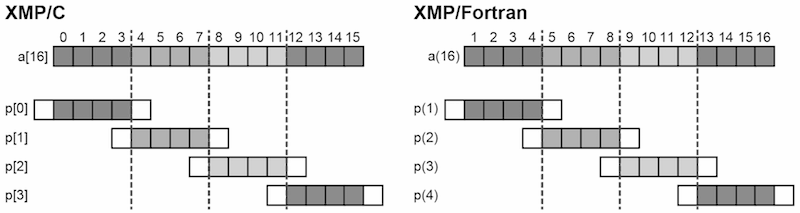
\includegraphics[width=\textwidth]{figs/shadow.png}
  \caption{Example of {\tt shadow} directive (1).}
\end{figure}

In the figure above, colored elements are those that each node owns and
white ones are shadow.

\begin{mynote}
  Arrays distributed in a cyclic manner cannot have shadow.  
\end{mynote}

%\paragraph{Widths of lower/upper bounds are different}

In some programs, it is natural that the widths of the shadow area on
the lower and upper bounds are different. There is also a case where the
shadow area exists only on either of the bounds. In the example below,
it is declared that a distributed array \|a| has a shadow area of width
one only on the upper bound.

\begin{XCexample}
#pragma xmp nodes p[4]
#pragma xmp template t[16]
#pragma xmp distribute t(block) onto p
double a[16];
#pragma xmp align a[i] with t[i]
#pragma xmp shadow a[0:1]
\end{XCexample}

\begin{XFexample}
!$xmp nodes p(4)
!$xmp template t(16)
!$xmp distribute t(block) onto p
real :: a(16)
!$xmp align a(i) with t(i)
!$xmp shadow a(0:1)
\end{XFexample}

\begin{figure}
  \centering
  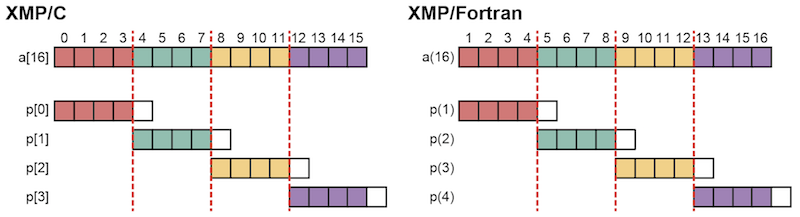
\includegraphics[width=\textwidth]{figs/shadow_uneven.png}
  \caption{Example of {\tt shadow} directive (2).}
\end{figure}

The values on the left- and right-hand sides of a colon designate the
widths on the lower and upper bounds, respectively.

\subsubsection{Updating Shadow}

%\paragraph{General}

To copy data to shadow areas from neighboring nodes, use the \|reflect|
construct. In the example below, the shadow areas of an array \|a| that
are of width one on both the upper and lower bounds are updated.

\begin{XCexample}
#pragma xmp reflect (a)

#pragma xmp loop on t[i]
for(int i=1;i<15;i++)
  a[i] = (a[i-1] + a[i] + a[i+1])/3;
\end{XCexample}

\begin{XFexample}
!$xmp reflect (a)

!xmp loop on t(i)
do i=2, 15
  a(i) = (a(i-1) + a(i) + a(i+1))/3
enddo
\end{XFexample}

\begin{figure}
  \centering
  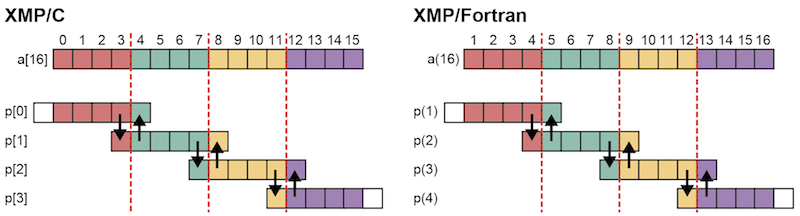
\includegraphics[width=\textwidth]{figs/reflect.png}
  \caption{Example of {\tt reflect} construct (1).}
\end{figure}

With this \|reflect| directive, in XMP/C, node \|p[1]| sends an element
\|a[4]| to the shadow area on the upper bound on node \|p[0]| and
\|a[7]| to the shadow area on the lower bound on \|p[2]|; \|p[0]| sends
an element \|a[3]| to the shadow area on the lower bound on \|p[1]|, and
\|p[2]| sends \|a[8]| to the shadow area on the upper bound on \|p[1]|.

Similarly, in XMP/Fortran, node \|p(2)| sends an element \|a(5)| to the
shadow area on the upper bound on node \|p(1)| and \|a(8)| to the shadow
area on the lower bound on \|p(3)|; \|p(1)| sends an element \|a(4)| to
the shadow area on the lower bound on \|p(2)|, and \|p(3)| sends \|a(9)|
to the shadow area on the upper bound on \|p(2)|.

%\paragraph{Specify Width}

The default behavior of a \|reflect| directive is to update the whole of
the shadow area declared by the \|shadow| directive. However, there are
some cases where a specific part of the shadow area is to be updated to
reduce the communication cost at a point of the code.

To update only a specific part of the shadow area, add the \|width|
clause to the \|reflect| directive.

The values on the left- and right-hand sides of a colon in the \|width|
clause designate the widths on the lower and upper bounds to be updated,
respectively. In the example below, only the shadow area on the upper
bound is updated.

\begin{XCexample}
#pragma xmp reflect (a) width(0:1)
\end{XCexample}

\begin{XFexample}
!$xmp reflect (a) width(0:1)
\end{XFexample}

\begin{figure}
  \centering
  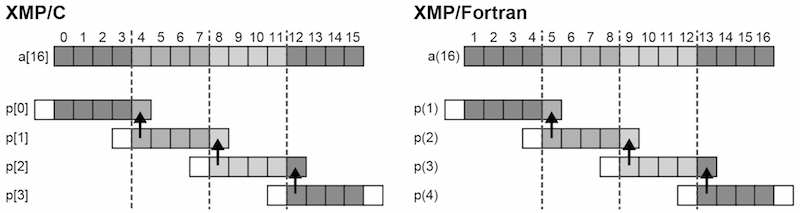
\includegraphics[width=\textwidth]{figs/reflect_width.png}
  \caption{Example of {\tt reflect} construct (2).}
\end{figure}

\begin{mynote}
  If the widths of the shadow areas to be updated on the upper and lower 
  bounds are equal, that is, for example, \|width(1:1)|, you can
  abbreviate it as \|width(1)|.
\end{mynote}

\begin{mynote}
  It is not possible to update the shadow area on a particular node
  because \|reflect| is a collective operation.
\end{mynote}

% If no shadow area is specified on the lower bound, the reflect directive
% does not update it with or without a width clause. The below figure
% illustrates the behavior of a reflect directive for a distributed array
% a having a shadow area of width one only on the upper bound.

% \begin{figure}
%   \centering
%   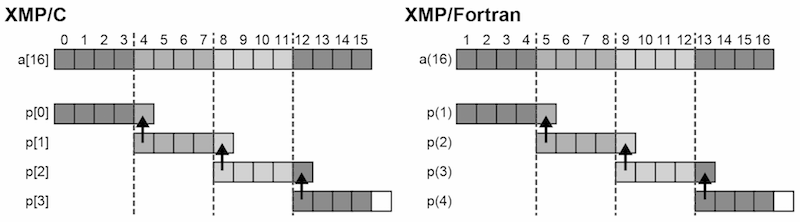
\includegraphics{figs/reflect_uneven.png}
% \end{figure}

%\paragraph{Update periodic shadow}

The \|reflect| directive does not update either the shadow area on the
lower bound on the leading node or that on the upper bound on the last
node. However, the values in such areas are needed for stencil
computation if periodic boundary conditions are used in the computation.

To update such areas, add a \|periodic| qualifier into the \|width|
clause. Let’s look at the following example where an array \|a| having
shadow areas of width one on both the lower and upper bounds appears.

\begin{XCexample}
#pragma xmp reflect (a) width(/periodic/1:1)
\end{XCexample}

\begin{XFexample}
!$xmp reflect (a) width(/periodic/1:1)
\end{XFexample}

\begin{figure}
  \centering
  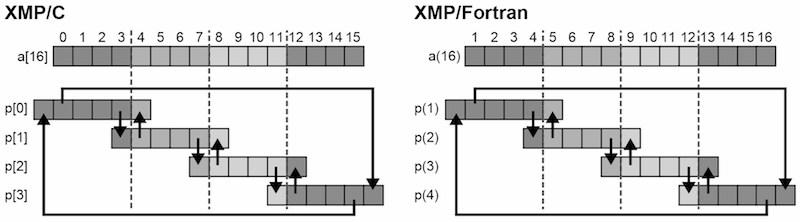
\includegraphics[width=\textwidth]{figs/reflect_periodic.png}
  \caption{Example of periodic {\tt reflect} construct.}
\end{figure}

The \|periodic| qualifier has the following effects, in addition to that of
a normal \|reflect| directive: in XMP/C, node \|p[0]| sends an element
\|a[0]| to the shadow area on the upper bound on node \|p[3]|, and
\|p[3]| sends \|a[15]| to the shadow area on the lower bound on \|p[0]|;
in XMP/Fortran, node \|p(1)| sends an element \|a(1)| to the shadow area
on the upper bound on node \|p(4)|, and \|p(4)| sends \|a(16)| to the
shadow area on the lower bound on \|p(1)|.

% \begin{mynote}
%   If the widths of the shadow areas to be updated on
% the upper and lower 
% bounds are equal, as shown by width(/periodic/1:1) in the above example,
% you can abbreviate it as width(/periodic/1).
% \end{mynote}

%\subsubsection{Multi-dimensional Shadow}

The \|shadow| directive and \|reflect| construct can be applied to
arrays distributed in multiple dimensions. The following programs are the
examples for two-dimensional distribution.

\begin{XCexample}
#pragma xmp nodes p[3][3]
#pragma xmp template t[9][9]
#pragma xmp distribute t[block][block] onto p
double a[9][9];
#pragma xmp align a[i][j] with t[i][j]
#pragma xmp shadow a[1][1]
   :
#pragma xmp reflect (a)
\end{XCexample}

\begin{XFexample}
!$xmp nodes p(3,3)
!$xmp template t(9,9)
!$xmp distribute t(block,block) onto p
real :: a(9,9)
!$xmp align a(j,i) with t(j,i)
!$xmp shadow a(1,1)
   :
!$xmp reflect (a)
\end{XFexample}

\begin{figure}
  \centering
  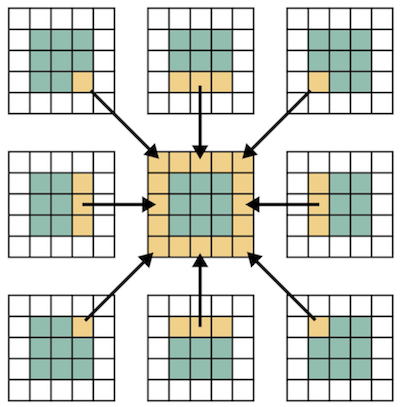
\includegraphics{figs/multi1.png}
  \caption{Example of multi-dimensional shadow (1).}
\end{figure}

The central node receives data from the surrounding eight
nodes to update its shadow areas. The shadow areas of the other nodes
are also updated, which is omitted in the figure.

For some applications, data from ordinal directions are not
necessary. In such a case, the data communication from/to the ordinal
directions can be avoided by adding the \|orthogonal| clause to a
\|reflect| construct.

\begin{XCexample}
#pragma xmp reflect (a) orthogonal
\end{XCexample}

\begin{XFexample}
!$xmp reflect (a) orthogonal
\end{XFexample}

\begin{figure}
  \centering
  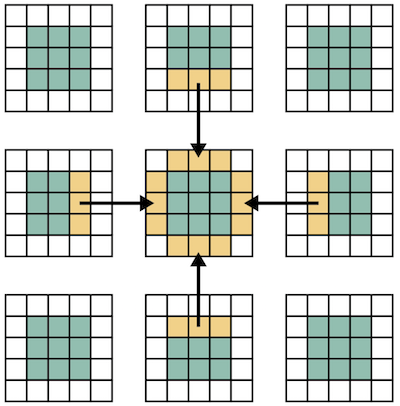
\includegraphics{figs/multi_orthogonal.png}
  \caption{Example of multi-dimensional shadow (2).}
\end{figure}

\begin{mynote}
  The \|orthogonal| clause is effective only for arrays
  more than one dimension of which is distributed.
\end{mynote}

Besides, you can also add shadow areas to only specified dimension.

\begin{XCexample}
#pragma xmp nodes p[3]
#pragma xmp template t[9]
#pragma xmp distribute t[block] onto p
double a[9][9];
#pragma xmp align a[i][*] with t[i]
#pragma xmp shadow a[1][0]
  :
#pragma xmp reflect (a)
\end{XCexample}

\begin{XFexample}
!$xmp nodes p[3]
!$xmp template t[9]
!$xmp distribute t[block] onto p
real :: a(9,9)
!$xmp align a(*,i) with t(i)
!$xmp shadow a(0,1)
  :
!$xmp reflect (a)
\end{XFexample}

\begin{figure}
  \centering
  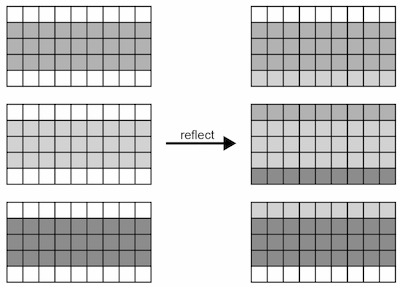
\includegraphics{figs/1of2.png}
  \caption{Example of multi-dimensional shadow (3).}
\end{figure}

For the array \|a|, 0 is specified as the shadow width in
non-distributed dimensions.


\subsection{{\tt gmove} Construct}

The programmaers can specify a communication of distributed arrays in
the form of assignment statements by using the \|gmove| construct.
%
In other words, with the \|gmove| construct, any array assignment
between two arrays (i.e. {\it global data movement}) that may involve
inter-node communication can be specified.

There are three modes of \|gmove|; ``collective mode,'' ``in mode,'' and
``out mode.''
% While collective mode executes two-sided communication among the
% executing nodes, in/out modes execute one-sided communication among
% tasks with a task directive. While in mode uses get communication, out
% mode uses put communication.

\subsubsection{Collective Mode}

%\paragraph{Distributed array}

% Copying a part of array a to array b. Array assignment statements in a
% gmove construct uses triplet.

The global data movement involved by a {\it collective} \|gmove| is performed
collectively, and results in implicit synchronization among the 
executing nodes.

\begin{XCexample}
#pragma xmp nodes p[4]
#pragma xmp template t[16]
#pragma xmp distribute t[block] onto p
int a[16], b[16];
#pragma xmp align a[i] with t[i]
#pragma xmp align b[i] with t[i]
     :
#pragma xmp gmove
  a[9:5] = b[0:5];
\end{XCexample}

\begin{XFexample}
!$xmp nodes p(4)
!$xmp template t(16)
!$xmp distribute t(block) onto p
integer :: a(16), b(16)
!$xmp align a(i) with t(i)
!$xmp align b(i) with t(i)
     :
!$xmp gmove
  a(10:14) = b(1:5)
\end{XFexample}

\begin{figure}
  \centering
  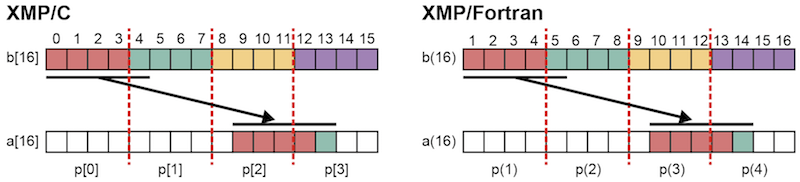
\includegraphics[width=\textwidth]{figs/gmove.png}
  \caption{Collective {\tt gmove} (1).}
\end{figure}

In XMP/C, \|p[0]| sends \|b[0]|-\|b[3]| to \|p[2]|-\|p[3]|, and \|p[1]|
sends \|b[4]| to \|p[3]|. Similarly, in XMP/Fortran, \|p(1)| sends
\|b(1)|-\|b(4)| to \|p(3)|-\|p(4)|, and \|p(2)| sends \|b(5)| to \|p(4)|.

\begin{XCexample}
#pragma xmp nodes p[4]
#pragma xmp template t1[16]
#pragma xmp template t2[16]
#pragma xmp distribute t1[cyclic] onto p
#pragma xmp distribute t2[block] onto p
int a[16], b[16];
#pragma xmp align a[i] with t1[i]
#pragma xmp align b[i] with t2[i]
     :
#pragma xmp gmove
  a[9:5] = b[0:5];
\end{XCexample}

\begin{XFexample}
!$xmp nodes p(4)
!$xmp template t1(16)
!$xmp template t2(16)
!$xmp distribute t1(cyclic) onto p
!$xmp distribute t2(block) onto p
integer :: a(16), b(16)
!$xmp align a(i) with t1(i)
!$xmp align b(i) with t2(i)
     :
!$xmp gmove
  a(10:14) = b(1:5)
\end{XFexample}

\begin{figure}
  \centering
  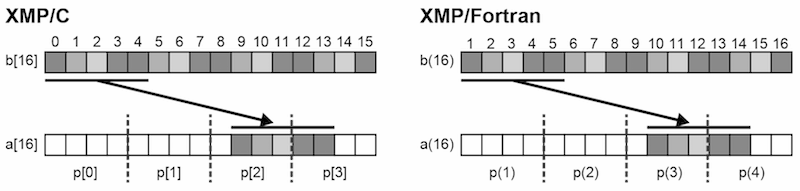
\includegraphics[width=\textwidth]{figs/gmove_cyclic.png}
  \caption{Collective {\tt gmove} (2).}
\end{figure}

While array \|a| is distributed in a cyclic manner, array \|b| is
distributed in a block manner.

In XMP/C, \|p[0]| sends \|b[0]| and \|b[4]| to \|p[2]| and
\|p[3]|. \|p[1]| sends \|b[1]| to \|p[2]|. Each element of \|p[2]| and
\|p[3]| will be copied locally. Similarly, in XMP/Fortran, \|p(1)| sends
\|b(1)| and \|b(5)| to \|p(3)| and \|p(4)|. \|p(2)| sends \|b(2)| to
\|p(3)|. Each element of \|p(3)| and \|p(4)| will be copied locally.

% \begin{mynote}
%   If the number of elements specified on the
% right-hand side is other than one, it will not work properly if the
%   number of elements differs between the right-hand side and the
%   left-hand side.
% \end{mynote}

By using this method, the distribution of an array can be ``changed''
during computation.

\begin{XCexample}
#pragma xmp nodes p[4]
#pragma xmp template t1[16]
#pragma xmp template t2[16]
int W[4] = {2,4,8,2};
#pragma xmp distribute t1[gblock(W)] onto p
#pragma xmp distribute t2[block] onto p
int a[16], b[16];
#pragma xmp align a[i] with t1[i]
#pragma xmp align b[i] with t2[i]
     :
#pragma xmp gmove
  a[:] = b[:];
\end{XCexample}

\begin{XFexample}
!$xmp nodes p(4)
!$xmp template t1(16)
!$xmp template t2(16)
integer :: W(4) = (/2,4,7,3/)
!$xmp distribute t1(gblock(W)) onto p
!$xmp distribute t2(block) onto p
integer :: a(16), b(16)
!$xmp align a(i) with t1(i)
!$xmp align b(i) with t2(i)
     :
!$xmp gmove
  a(:) = b(:)
\end{XFexample}

\begin{figure}
  \centering
  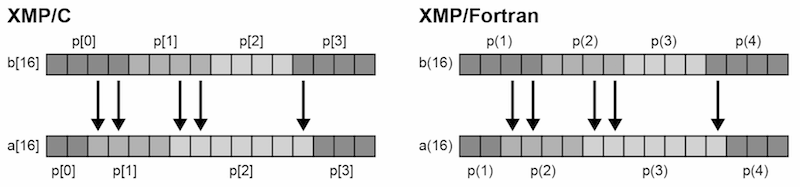
\includegraphics[width=\textwidth]{figs/gmove_change.png}
  \caption{Collective {\tt gmove} (3).}
\end{figure}

In this example, the elements of an array \|b| that is distributed in
a block manner are copied to the corresponding elements of an array \|a|
that is distributed in a generalized-block manner.
%
For the arrays \|a| and \|b|, communication occurs if corresponding elements
reside in different nodes (arrows illustrate communication between nodes in
the figures).

%\paragraph{Scalar}

In the assignment statement, if a scalar (i.e. one element of an array or
a variable) is specified on the right-hand side and an array section are
specified on the left-hand side, a broadcast communication occurs for it.

\begin{XCexample}
#pragma xmp nodes p[4]
#pragma xmp template t[16]
#pragma xmp distribute t[block] onto p
int a[16], b[16];
#pragma xmp align a[i] with t[i]
#pragma xmp align b[i] with t[i]
     :
#pragma xmp gmove
  a[9:5] = b[0];
\end{XCexample}

\begin{XFexample}
!$xmp nodes p(4)
!$xmp template t(16)
!$xmp distribute t(block) onto p
integer :: a(16), b(16)
!$xmp align a(i) with t(i)
!$xmp align b(i) with t(i)
     :
!$xmp gmove
  a(10:14) = b(1)
\end{XFexample}

\begin{figure}
  \centering
  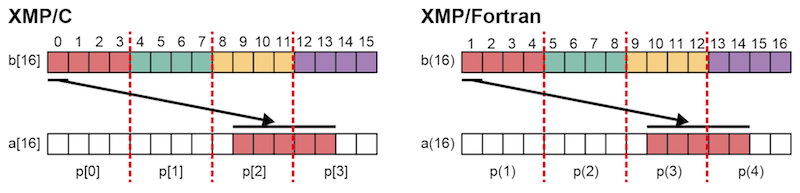
\includegraphics[width=\textwidth]{figs/gmove_one_element.png}
  \caption{Collective {\tt gmove} (4).}
\end{figure}

In this example, in XMP/C, an array element \|b[0]| of node \|p[0]| will be
broadcasted to the specified array section on node \|p[2]| and
\|p[3]|. Similarly, in XMP/Fortran, an array element \|b(1)| of node
\|p(1)| will be broadcasted to the specified array section on node \|p(3)| and \|p(4)|.

%\paragraph{Duplicated array and scalar}

Not only distributed arrays but also replicated arrays can be specified
on the right-hand side.

\begin{XCexample}
 #pragma xmp nodes p[4]
 #pragma xmp template t[16]
 #pragma xmp distribute t[block] onto p
 int a[16], b[16], c;
 #pragma xmp align a[i] with t[i]
      :
#pragma xmp gmove
   a[9:5] = b[0:5];
\end{XCexample}

\begin{XFexample}
 !$xmp nodes p(4)
 !$xmp template t(16)
 !$xmp distribute t(block) onto p
 integer :: a(16), b(16), c
 !$xmp align a(i) with t(i)
      :
!$xmp gmove
   a(10:14) = b(1:5)
\end{XFexample}

In this example, a replicated array \|b| is locally copied to
distributed array \|a| without communication.

%\paragraph{Distributed array with different dimension}

\begin{XCexample}
#pragma xmp nodes p[4]
#pragma xmp template t1[8]
#pragma xmp template t2[16]
#pragma xmp distribute t1[block] onto p
#pragma xmp distribute t2[block] onto p
int a[8][16], b[8][16];
#pragma xmp align a[i][*] with t1[i]
#pragma xmp align b[*][i] with t2[i]
     :
#pragma xmp gmove
  a[0][:] = b[0][:];
\end{XCexample}

\begin{XFexample}
!$xmp nodes p(4)
!$xmp template t1(8)
!$xmp template t2(16)
!$xmp distribute t1(block) onto p
!$xmp distribute t2(block) onto p
integer :: a(16,8), b(8,16)
!$xmp align a(*,i) with t1(i)
!$xmp align b(i,*) with t2(i)
     :
#pragma xmp gmove
  a(:,1) = b(:,1)
\end{XFexample}

\begin{figure}
  \centering
  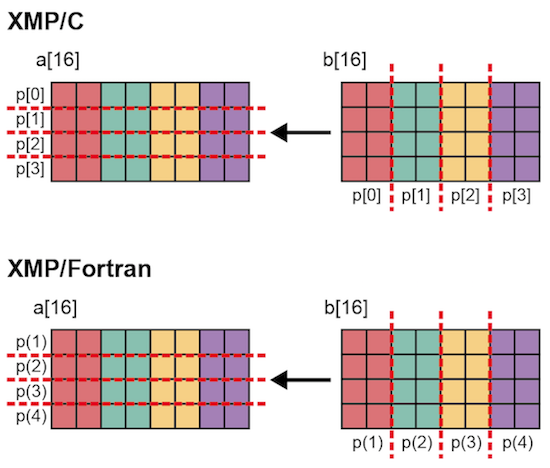
\includegraphics{figs/gmove_different.png}
  \caption{Collective {\tt gmove} (4).}
\end{figure}

In this example, in XMP/C, \|b[0][0:2]| on \|p[0]|, \|b[0][2:2]| of
\|p[1]|, \|b[0][4:2]| on \|p[2]| and \|b[0][6:2]| on \|p[3]| are copied
to \|a[0][:]| on \|p[0]|. Similarly, in XMP/Fortran, \|b(1:2,1)| on
\|p(1)|, \|b(3:4,1)| of \|p(2)|, \|b(5:6,1)| on \|p(3)| and \|b(7:8,1)|
on \|p(4)| are copied to \|a(:,1)| on \|p(1)|.


\subsubsection{In Mode}

%It operates as in mode by setting in clause to gmove directive.

The right-hand side data of the assignment, all or part of which may
reside outside the executing node set, can be transferred from its owner
nodes to the executing nodes with an {\it in} \|gmove|.

\begin{XCexample}
#pragma xmp nodes p[4]
#pragma xmp template t[4]
#pragma xmp distribute t[block] onto p
double a[4], b[4];
#pragma xmp align a[i] with t[i]
#pragma xmp align b[i] with t[i]
   :
#pragma xmp task on p[0:2]
#pragma xmp gmove in
  a[0:2] = b[2:2]
#pragma xmp end task
\end{XCexample}

\begin{XFexample}
!$xmp nodes p(4)
!$xmp template t(4)
!$xmp distribute t(block) onto p
real :: a(4), b(4)
!$xmp align a(i) with t(i)
!$xmp align b(i) with t(i)
   :
!$xmp task on p(1:2)
!$xmp gmove in
  a(1:2) = b(3:4)
!$xmp end task
\end{XFexample}

In this example, the \|task| directive divides four nodes into
two sets, the first-half and the second-half. A \|gmove| construct that
is in an {\it in} mode copies data using a {\it get} operation from
the second-half node to the first-half node.

\begin{figure}
  \centering
  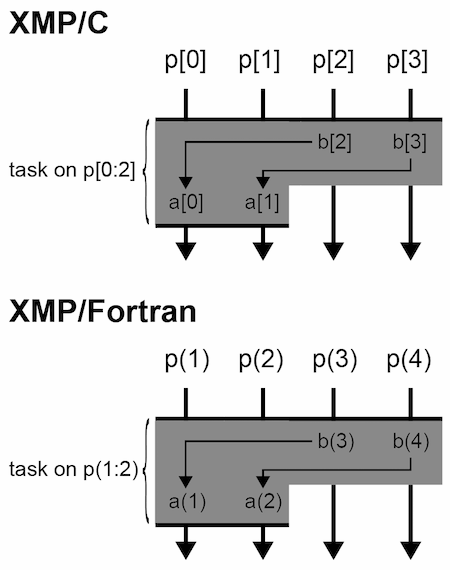
\includegraphics{figs/gmove_in.png}
  \caption{In {\tt gmove}.}
\end{figure}


\subsubsection{Out Mode}

For the left-hand side data of the assignment, all or part of which may
reside outside the executing node set, the corresponding elements can be
transferred from the executing nodes to its owner nodes with an {\it out}
\|gmove| construct.

\begin{XCexample}
#pragma xmp nodes p[4]
#pragma xmp template t[4]
#pragma xmp distribute t[block] onto p
double a[4], b[4];
#pragma xmp align a[i] with t[i]
#pragma xmp align b[i] with t[i]
   :
#pragma xmp task on p[0:2]
#pragma xmp gmove out
  b[2:2] = a[0:2]
#pragma xmp end task
\end{XCexample}

\begin{XFexample}
!$xmp nodes p(4)
!$xmp template t(4)
!$xmp distribute t(block) onto p
real :: a(4), b(4)
!$xmp align a(i) with t(i)
!$xmp align b(i) with t(i)
   :
!$xmp task on p(1:2)
!$xmp gmove out
  b(3:4) = a(1:2)
!$xmp end task
\end{XFexample}

A \|gmove| construct that is in {\it out} mode copies data using a {\it put}
communication from the first-half nodes to the second-half nodes.

\begin{figure}
  \centering
  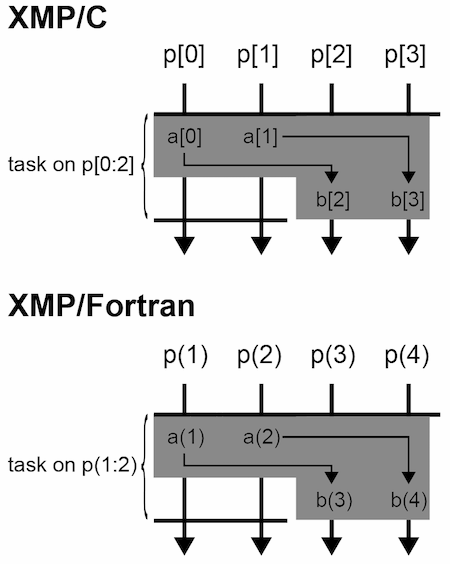
\includegraphics{figs/gmove_out.png}
  \caption{Out {\tt gmove}.}
\end{figure}


\subsection{{\bf barrier} Construct}

The \|barrier| construct executes a barrier synchronization.

\begin{XCexample}
#pragma xmp barrier
\end{XCexample}

\begin{XFexample}
!$xmp barrier
\end{XFexample}

You can specify a node set on which the barrier synchroniation is to be
performed by using the \|on| clause. In the below example, a barrier
synchronization is performed among the first two nodes of \|p|.

\begin{XCexample}
#pragma xmp barrier on p[0:2]
\end{XCexample}

\begin{XFexample}
!$xmp barrier on p(1:2)
\end{XFexample}


\subsection{{\bf reduction} Construct}

This construct performs a {\it reduction} operation. It has the same
meaning as the \|reduction| clause of the \|loop| construct, but this
construct can be specified anywhere as an {\it executable} construct.

\begin{XCexample}
#pragma xmp nodes p[4]
  :
sum = xmpc_node_num() + 1;
#pragma xmp reduction (+:sum)
\end{XCexample}

\begin{XFexample}
!$xmp nodes p(4)
  :
sum = xmp_node_num()
!$xmp reduction (+:sum)
\end{XFexample}

\begin{figure}
  \centering
  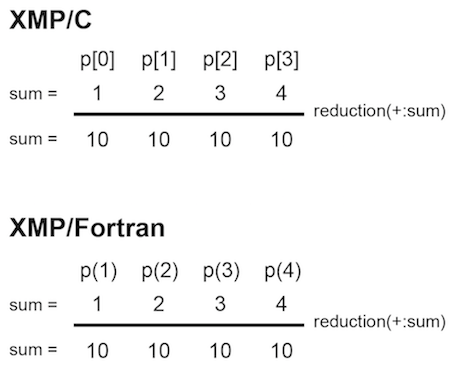
\includegraphics{figs/reduction.png}
  \caption{{\tt reduction} construct (1).}
\end{figure}

You can specify the executing node set by using the \|on| clause. In the
below example, only the values on the last two of the four nodes are
targeted by the \|reduction| construct.

\begin{XCexample}
#pragma xmp nodes p[4]
  :
sum = xmpc_node_num() + 1;
#pragma xmp reduction (+:sum) on p[2:2]
\end{XCexample}

\begin{XFexample}
!$xmp nodes p(4)
  :
 sum = xmp_node_num()
 !$xmp reduction (+:sum) on p(3:4)
\end{XFexample}

\begin{figure}
  \centering
  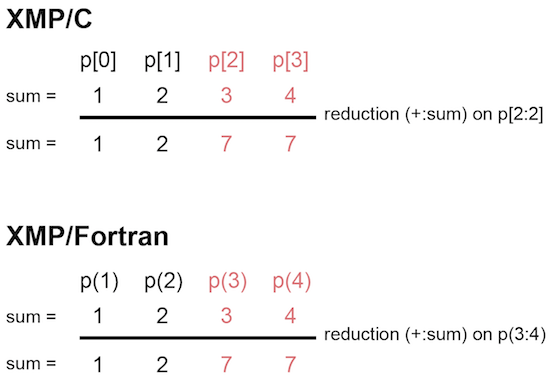
\includegraphics{figs/reduction_on.png}
  \caption{{\tt reduction} construct (2).}
\end{figure}

The operators you can use in the \|reduction| construct are as follows:

\begin{XCexample}
+
*
-
&
|
^
&&
||
max
min
\end{XCexample}

\begin{XFexample}
+
*
-
.and.
.or.
.eqv.
.neqv.
max
min
iand
ior
ieor
\end{XFexample}

\begin{mynote}
% Since the \|reduction| clause needs a loop statement,
% operators of
% firstmax, firstmin, lastmax, and lastmin are required. But, since the
% reduction directive does not need a loop statement, there are no such
% operators.
  In contrast to the \|reduction| clause of the \|loop| construct, which
  precedes loops, the \|reduction| construct does not accept operators of
  \|firstmax|, \|firstmin|, \|lastmax|, and \|lastmin|.
\end{mynote}

\begin{mynote}
  Similar to the \|reduction| clause, the \|reduction| construct may
  generate slightly different results in a parallel execution from those
  in a sequential execution, because the results depends on the order of
  combining the value.
\end{mynote}


\subsection{{\bf bcast} Construct}

The \|bcast| construct broadcasts the values of the variables on the
node specified by the \|from| clause, that is, the {\it root node}, to
the node set specified by the \|on| clause.
%
If there is no \|from| clause, the first node of the executing node
set is selected as the root node.
%
If there is no \|on| clause, the current executing node set of the
construct is selected as the executing node set.

In the below example, the first node of the node set \|p|, that is,
\|p[0]| or \|p(1)|, is the root node.

\begin{XCexample}
#pragma xmp nodes p[4]
  :
num = xmpc_node_num() + 1;
#pragma xmp bcast (num)
\end{XCexample}

\begin{XFexample}
!$xmp nodes p(4)
  :
num = xmp_node_num()
!$xmp bcast (num)
\end{XFexample}

\begin{figure}
  \centering
  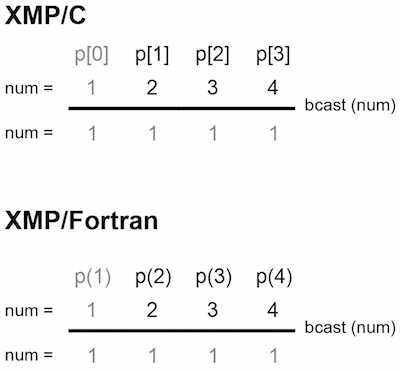
\includegraphics{figs/bcast.png}
  \caption{{\tt bcast} construct (1).}
\end{figure}

In the below example, the last node, that is, \|p[3]| or \|p(4)|, is the \|from| clause.

\begin{XCexample}
#pragma xmp nodes p[4]
  :
num = xmpc_node_num() + 1;
#pragma xmp bcast (num) from p[3]
\end{XCexample}

\begin{XFexample}
!$xmp nodes p(4)
  :
num = xmp_node_num()
!$xmp bcast (num) from p(4)
\end{XFexample}

\begin{figure}
  \centering
  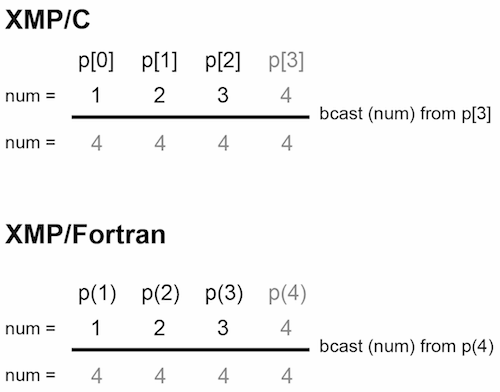
\includegraphics{figs/bcast_from.png}
  \caption{{\tt bcast} construct (2).}
\end{figure}

In the below example, only the last three of four nodes
are included by the executing node set of the \|bcast| construct.

\begin{XCexample}
#pragma xmp nodes p[4]
  :
sum = xmpc_node_num() + 1;
#pragma xmp bcast (num) from p[3] on p[1:3]
\end{XCexample}

\begin{XFexample}
!$xmp nodes p(4)
  :
 sum = xmp_node_num()
 !$xmp bcast (num) from p(4) on p(2:4)
\end{XFexample}

\begin{figure}
  \centering
  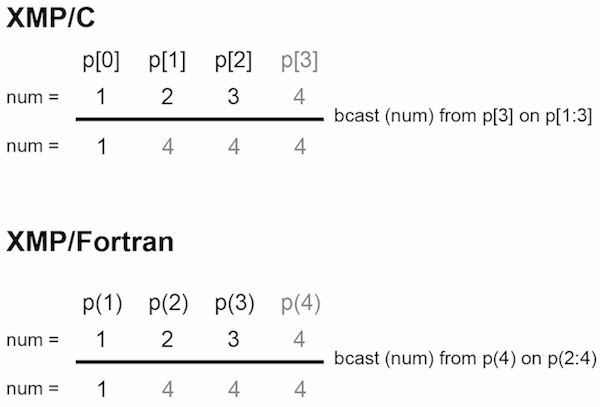
\includegraphics{figs/bcast_from_on.png}
  \caption{{\tt bcast} construct (3).}
\end{figure}


\subsection{{\bf wait\_async} Construct}

Communication directives (i.e. \|reflect|, \|gmove|, \|reduction|,
\|bcast|, and \|reduce_shadow|) can perform asynchronous communication if
the \|async| clause is added. The \|wait_async| construct is used to
guarantee the completion of such an asynchronous communication.

\begin{XCexample}
#pragma xmp bcast (num) async(1)
    :
#pragma xmp wait_async (1)
\end{XCexample}

\begin{XFexample}
!$xmp bcast (num) async(1)
        :
!$xmp wait_async (1)
\end{XFexample}

Since the \|bcast| directive has an \|async| clause, communication may
not be completed immediately after the \|bcast| directive. The
completion of that communication is guaranteed with the \|wait_async|
construct having the same value as that of the \|async| clause.
%
Therefore, between the \|bcast| construct and the \|wait_async|
constructs, you may not reference the target variable of the \|bcast|
directive.

\begin{myhint}
  Asynchronous communication can be overlapped with the following
  computation to hide its overhead.
\end{myhint}

\begin{mynote}
  Expressions that can be specified as {\it tags} in the \|async| clause are
  of type int, in XMP/C, or integer, in XMP/Fortran.
\end{mynote}


\subsection{{\bf reduce\_shadow} Construct}

The \|reduce_shadow| directive adds the value of a shadow object to the
corresponding data object of the array.

\begin{XCexample}
#pragma xmp nodes p[2]
#pragma xmp template t[8]
#pragma xmp distribute t[block] onto p
int a[8];
#pragma xmp align a[i] with t[i]
#pragma xmp shadow a[1]
 :
#pragma xmp loop on t[i]
  for(int i=0;i<8;i++)
    a[i] = i+1;

#pragma xmp reflect (a)
#pragma xmp reduce_shadow (a)
\end{XCexample}

\begin{XFexample}
!$xmp nodes p(2)
!$xmp template t(8)
!$xmp distribute t(block) onto p
  integer a(8)
!$xmp align a(i) with t(i)
!$xmp shadow a(1)

!$xmp loop on t(i)
  do i=1, 8
    a(i) = i
  enddo

!$xmp reflect (a)
!$xmp reduce_shadow (a)
\end{XFexample}

% The \|shadow| directive adds a shadow are of width one to the
% distributed array \|a| of each node. Next, the \|reflect| construct
% updates the shadow area. Finally, the \|reduce_shadow| construct adds
% the value of the shadow to the value of the source element.

For the above example, in XMP/C, \|a[3]| on \|p[0]| has a value of eight,
and \|a[4]| on \|p[1]| has a value of ten. Similarly, in XMP/Fortran,
\|a(4)| of \|p(1)| has a value of eight, and \|a(5)| on \|p(2)| has a
value of ten.

\begin{figure}
  \centering
  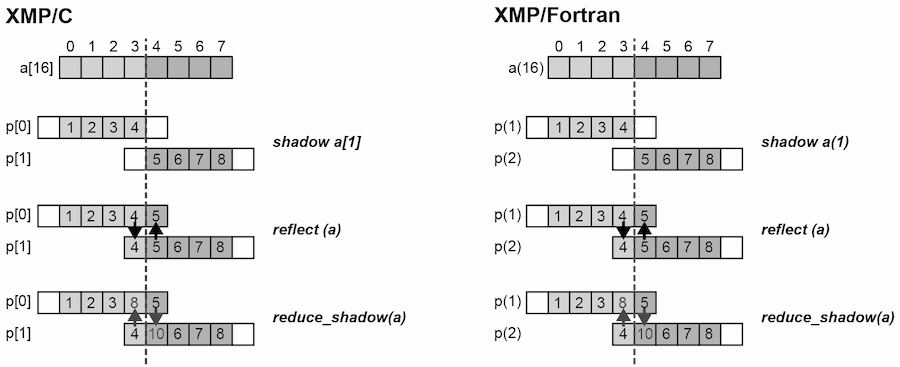
\includegraphics[width=\textwidth]{figs/reduce_shadow.png}
  \caption{{\tt reduce\_shadow} construct (1).}
\end{figure}

The programmers can add the \|periodic| modifier to the \|width| clause
to reduce shadow objects to the corresponding data object periodically.

\begin{XCexample}
#pragma xmp reflect (a) width(/periodic/1)
#pragma xmp reduce_shadow (a) width(/periodic/1)
\end{XCexample}

\begin{XFexample}
!$xmp reflect (a) width(/periodic/1)
!$xmp reduce_shadow (a) width(/periodic/1)
\end{XFexample}

\begin{figure}
  \centering
  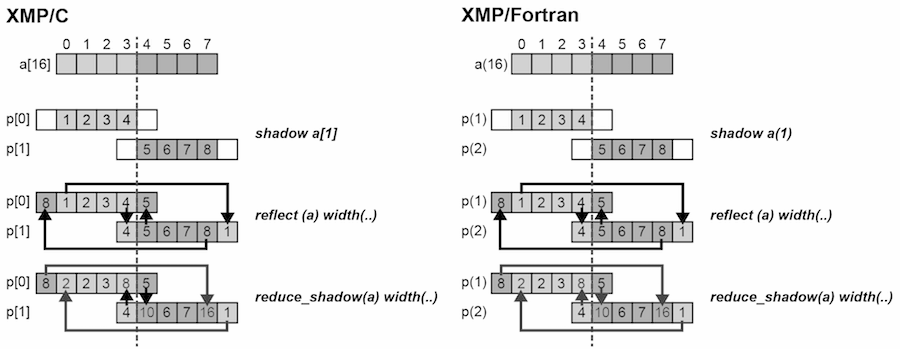
\includegraphics[width=\textwidth]{figs/reduce_shadow_periodic.png}
  \caption{{\tt reduce\_shadow} construct (2).}
\end{figure}

In addition to the first example, in XMP/C, \|a[0]| on \|p[0]| has a
value of two, and \|a[7]| on \|p[1]| has a value of 16. Similarly, in
XMP/Fortran, \|a(1)| in \|p(1)| has a value of two, and \|a(8)| in
\|p(2)| has a value of 16.